% Copyright 2019 by an anonymous contributor
%
% This file may be distributed and/or modified
%
% 1. under the LaTeX Project Public License and/or
% 2. under the GNU Free Documentation License.
%
% See the file doc/generic/pgf/licenses/LICENSE for more details.


\section{Bounding Boxes for B\'ezier Curves}

\begin{pgflibrary}{bbox}
    This library provides methods to determine tight bounding boxes for
    B\'ezier curves.
\end{pgflibrary}


\subsection{Current Status}

\tikzname\ determines the bounding box of (cubic) B\'ezier curves by
establishing the smallest rectangle that contains the end point and the two
control points of the curve.  This may lead to drastic overestimates of the
bounding box.

\begin{codeexample}[]
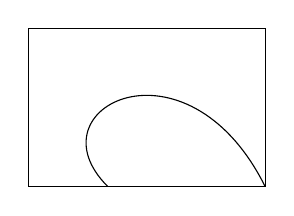
\begin{tikzpicture}
  \draw (0,0) .. controls (-1,1) and (1,2) .. (2,0);
  \draw (current bounding box.south west) rectangle
    (current bounding box.north east);
\end{tikzpicture}
\end{codeexample}

\subsection{Computing the Bounding Box}

Establishing the precise bounding box has been discussed in various places, the
following discussion uses in part the results from
\url{https://pomax.github.io/bezierinfo/}. What is a cubic Bezier curve? A
cubic Bezier curve running from $(x_0,y_0)$ to $(x_1,y_1)$ with control points
$(x_a,y_a)$ and $(x_a,y_a)$ can be parametrized by
\begin{equation}
 \gamma(t) =
 \begin{pmatrix} x(t)\\ y(t) \end{pmatrix} =
 \begin{pmatrix}t^3 x_{1}+3 t^2 (1-t) x_{b}+(1-t)^3
   x_{0}+3 t (1-t)^2 x_{a}\\
   t^3 y_{1}+3
   t^2 (1-t) y_{b}+(1-t)^3 y_{0}+3 t (1-t)^2
   y_{a}\end{pmatrix}\;,\label{eq:gammaBezier}
\end{equation}
where $t$ runs from 0 to 1 (and $\gamma(0)=(x_0,y_0)$ and
$\gamma(1)=(x_1,y_1)$). Surely, the bounding box has to contain
$(x_0,y_0)$ and $(x_1,y_1)$. If the functions $x(t)$ and $y(t)$ have extrema in
the interval $[0,1]$, then the bounding box will in general be larger than that.
In order to determine the extrema of the curve, all
we need to find the extrema of the functions $x(t)$ and $y(t)$ for $0\le t\le
1$. That is, we need to find the solutions of the quadratic equations
\begin{equation}
 \frac{\mathrm{d}x}{\mathrm{d}t}(t) = 0\quad\text{and}\quad
 \frac{\mathrm{d}y}{\mathrm{d}t}(t) = 0\;.
\end{equation}
Let's discuss $x$, $y$ is analogous. If the discriminant
\begin{equation}
 d := (x_a-x_b)^2+(x_1-x_b)(x_0-x_a)
\end{equation}
is greater than 0, there are two solutions
\begin{equation}
 t_\pm = \frac{x_{0}-2
   x_{a}+x_{b}\pm\sqrt{d}}{x_{0}-x_{1}-3(x_{a}- x_{b})} \;.
\end{equation}
In this case, we need to make sure that the bounding box contains, say
$(x(t_-),y_0)$ and $(x(t_+),y_0)$. If $d\le0$, the bounding box does not need to
be increased in the $x$ direction. One can plug $t_\pm$ back into
\eqref{eq:gammaBezier}, this yields
\begin{subequations}
\begin{align}
    x_- &=
    \!\begin{aligned}[t]
        \frac{1}{(x_0 - x_1 - 3x_a + 3x_b)^2}
        \Bigl[
            & x_0^2x_1 + x_0x_1^2 - 3x_0x_1x_a + 6x_1x_a^2
              + 2x_a^3 - 3(x_0 + x_a)(x_1 + x_a)x_b \\
            & + 3(2x_0 - x_a)x_b^2 + 2x_b^3
              - 2\sqrt{d}(x_0x_1 - x_1x_a + x_a^2 - (x_0 + x_a)x_b + x_b^2)
        \Bigr],
    \end{aligned} \\
    x_+ &=
    \!\begin{aligned}[t]
        \frac{1}{(x_0 - x_1 - 3x_a + 3x_b)^2}
        \Bigl[
            & x_0^2x_1 + x_0x_1^2 - 3x_0x_1x_a + 6x_1x_a^2
              + 2x_a^3 - 3(x_0 + x_a)(x_1 + x_a)x_b \\
            & + 3(2x_0 - x_a)x_b^2 + 2x_b^3
              + 2\sqrt{d}(x_0x_1 - x_1x_a + x_a^2 - (x_0 + x_a)x_b + x_b^2)
        \Bigr].
    \end{aligned}
\end{align}
\end{subequations}
As already mentioned, the analogous
statements apply to $y(t)$.

This procedure is implemented in the |bbox| library.  It installs a single key
by which the tight bounding box algorithm can be turned on and off.

\begin{key}{/pgf/bezier bounding box=\meta{boolean} (default true)}
    Turn the tight bounding box algorithm on and off.

    \emph{Caveat:} As can be seen from the derivations, the necessary
    computations involve the squaring of lengths, which can easily lead to
    |dimension too large| errors.  The library tries to account for large
    numbers by appropriate normalization, such that it works in most cases, but
    errors may still occur.
\end{key}

\begin{codeexample}[]
\begin{tikzpicture}[bezier bounding box=true]
  \draw (0,0) .. controls (-1,1) and (1,2) .. (2,0);
  \draw (current bounding box.south west) rectangle
    (current bounding box.north east);
\end{tikzpicture}
\end{codeexample}


%%% Local Variables:
%%% mode: latex
%%% TeX-master: "pgfmanual-pdftex-version"
%%% End:
